%preamble
\documentclass[letterpaper]{article}
\synctex=1
\usepackage{graphicx}
\graphicspath{ {images/} }

\usepackage{lipsum}
\usepackage{float}
% \bibliographystyle{IEEEtran}
\bibliographystyle{ieeetr}

\usepackage{amssymb}

\usepackage{siunitx}
%actual document
\begin{document}

  % \maketitle %insert titlepage here
  \begin{titlepage}
    \begin{center}
        \vspace*{1cm}
        \Huge
        Experiment 4
        \vspace{1cm}

        Magnetic Fields
        \vspace{1cm}

        By: Arun Woosaree
        \vspace{1cm}

        Lab partners:
        \vspace{.25cm}
        \Large

        Fatemeh Ghafari Far\\
        % Purvish Jajal
        \vspace{.25cm}
        Yvonne Hong
        \vspace{1cm}

        \Huge
        PHYS 230 Lab EH71
        \vspace{1cm}

        TA: Andrei Tretiakov
        \vspace{1cm}

        Date of Lab: March 22, 2018%\today
        \vfill
    \end{center}
\end{titlepage}

\section{Introduction}
% Begin with experiment’s objectives\\
% Give physical background:\\
% ○ Describe investigated/used\\
% phenomena e.g. Gauss’s law,\\
% field lines, equipotential lines.\\
% ○ Do not copy text from a
% textbook/manual\\
% Provide equations you used\\
% ○ Identify all symbols\\

In this experiment, we measure the distribution of the magnetic field across a solenoid.
The right hand rule is used to determine the
direction of the magnetic $\textbf{B}$ field in the coils of wire. The right handed rule
is defined as follows: the four main fingers of one's right hand curls in the direction of the
current in the wire, and the resulting direction in which the thumb points is the direction of the
$\textbf{B}$ field. By taking measurements of the earth's magnetic field $B_E$, and some physical measurements
of the coils, such as the solenoid length $L$, its radius $R$, and number of turns $N$, we gain insight
on how the magnetic field inside a solenoid with current running through it behaves.

\begin{equation}
  B=\frac{1}{2}\mu_0nI(\cos{\beta_2}-\cos{\beta_1})
\end{equation}
where $\mu_0=\SI{4\pi e-7}{\henry\per\metre}$ is the magnetic permeability of free space,
$n=N/L$ is the number of turns per unit length of the solenoid, $I$ is the current in the coil, and the cosine
arguments are shown in Figure 1. \textbf{NOT FIGURE 1 FIX THIS BUT IDK WHAT FIGURE IT IS YET BECAUSE I DIDN'T WRITE THAT PART OF THE LAB REPORT YET}

We also measure the magnetic field of a Helmholtz coil, from which we experimentally determine the
number of turns of the wire in the coil using the following equations and by plotting a graph.
\begin{equation}
  B_c=\frac{\frac{1}{2}\mu_0NR^2I}{(R^2+(x-x_c)^2)^{\frac{3}{2}}}
\end{equation}
where $N$ is the number of turns, $R$ is the coil radius, $I$ is the current,
$x$ is the position along the central axis, and $x_c$ is the center position of the coil.
In our setup, we have two identical coils with the same centre axis, separated by a
distance equivalent to radius $R$. This arrangement is called a Helmholtz coil,
and the magnetic field along the axis halfway between the fields is given by:
\begin{equation}
  B_H=\frac{8\mu_0NI}{\sqrt{125}R}
\end{equation}
where $B_H$ is the magnitude of the Helmholtz magnetic field.
From the above equations, we also obtain
expressions for $B_c$, the magnetic field in the center of a single coil, and
a simplified expression for $B_s$, in the center of a real solenoid.

\section{Experimental Method}
% List all equipment used\\
% ○ Provide parameters as detailed as
% possible: masses, frequencies,
% etc.\\
% Report what YOU DID to achieve
% experimental goals:\\
% ○ Do not use imperative clause\\
% ○ Use first person narrative or
% passive voice\\
% Based on this section you should be
% able to reproduce your results without a
% manual

%use p1-2 and p2-3 to show setup


\textbf{List of Equipment:}
\begin{itemize}
  \item Solenoid Coil
  \item Helmholtz Coil
  \item DC Power Supply with variable current
  \item Switch
  \item Banana Plug Wires
  \item Hall Probe apparatus with LoggerPro software
\end{itemize}

\subsection{Part 1}

\begin{figure}[H]
    \centering
    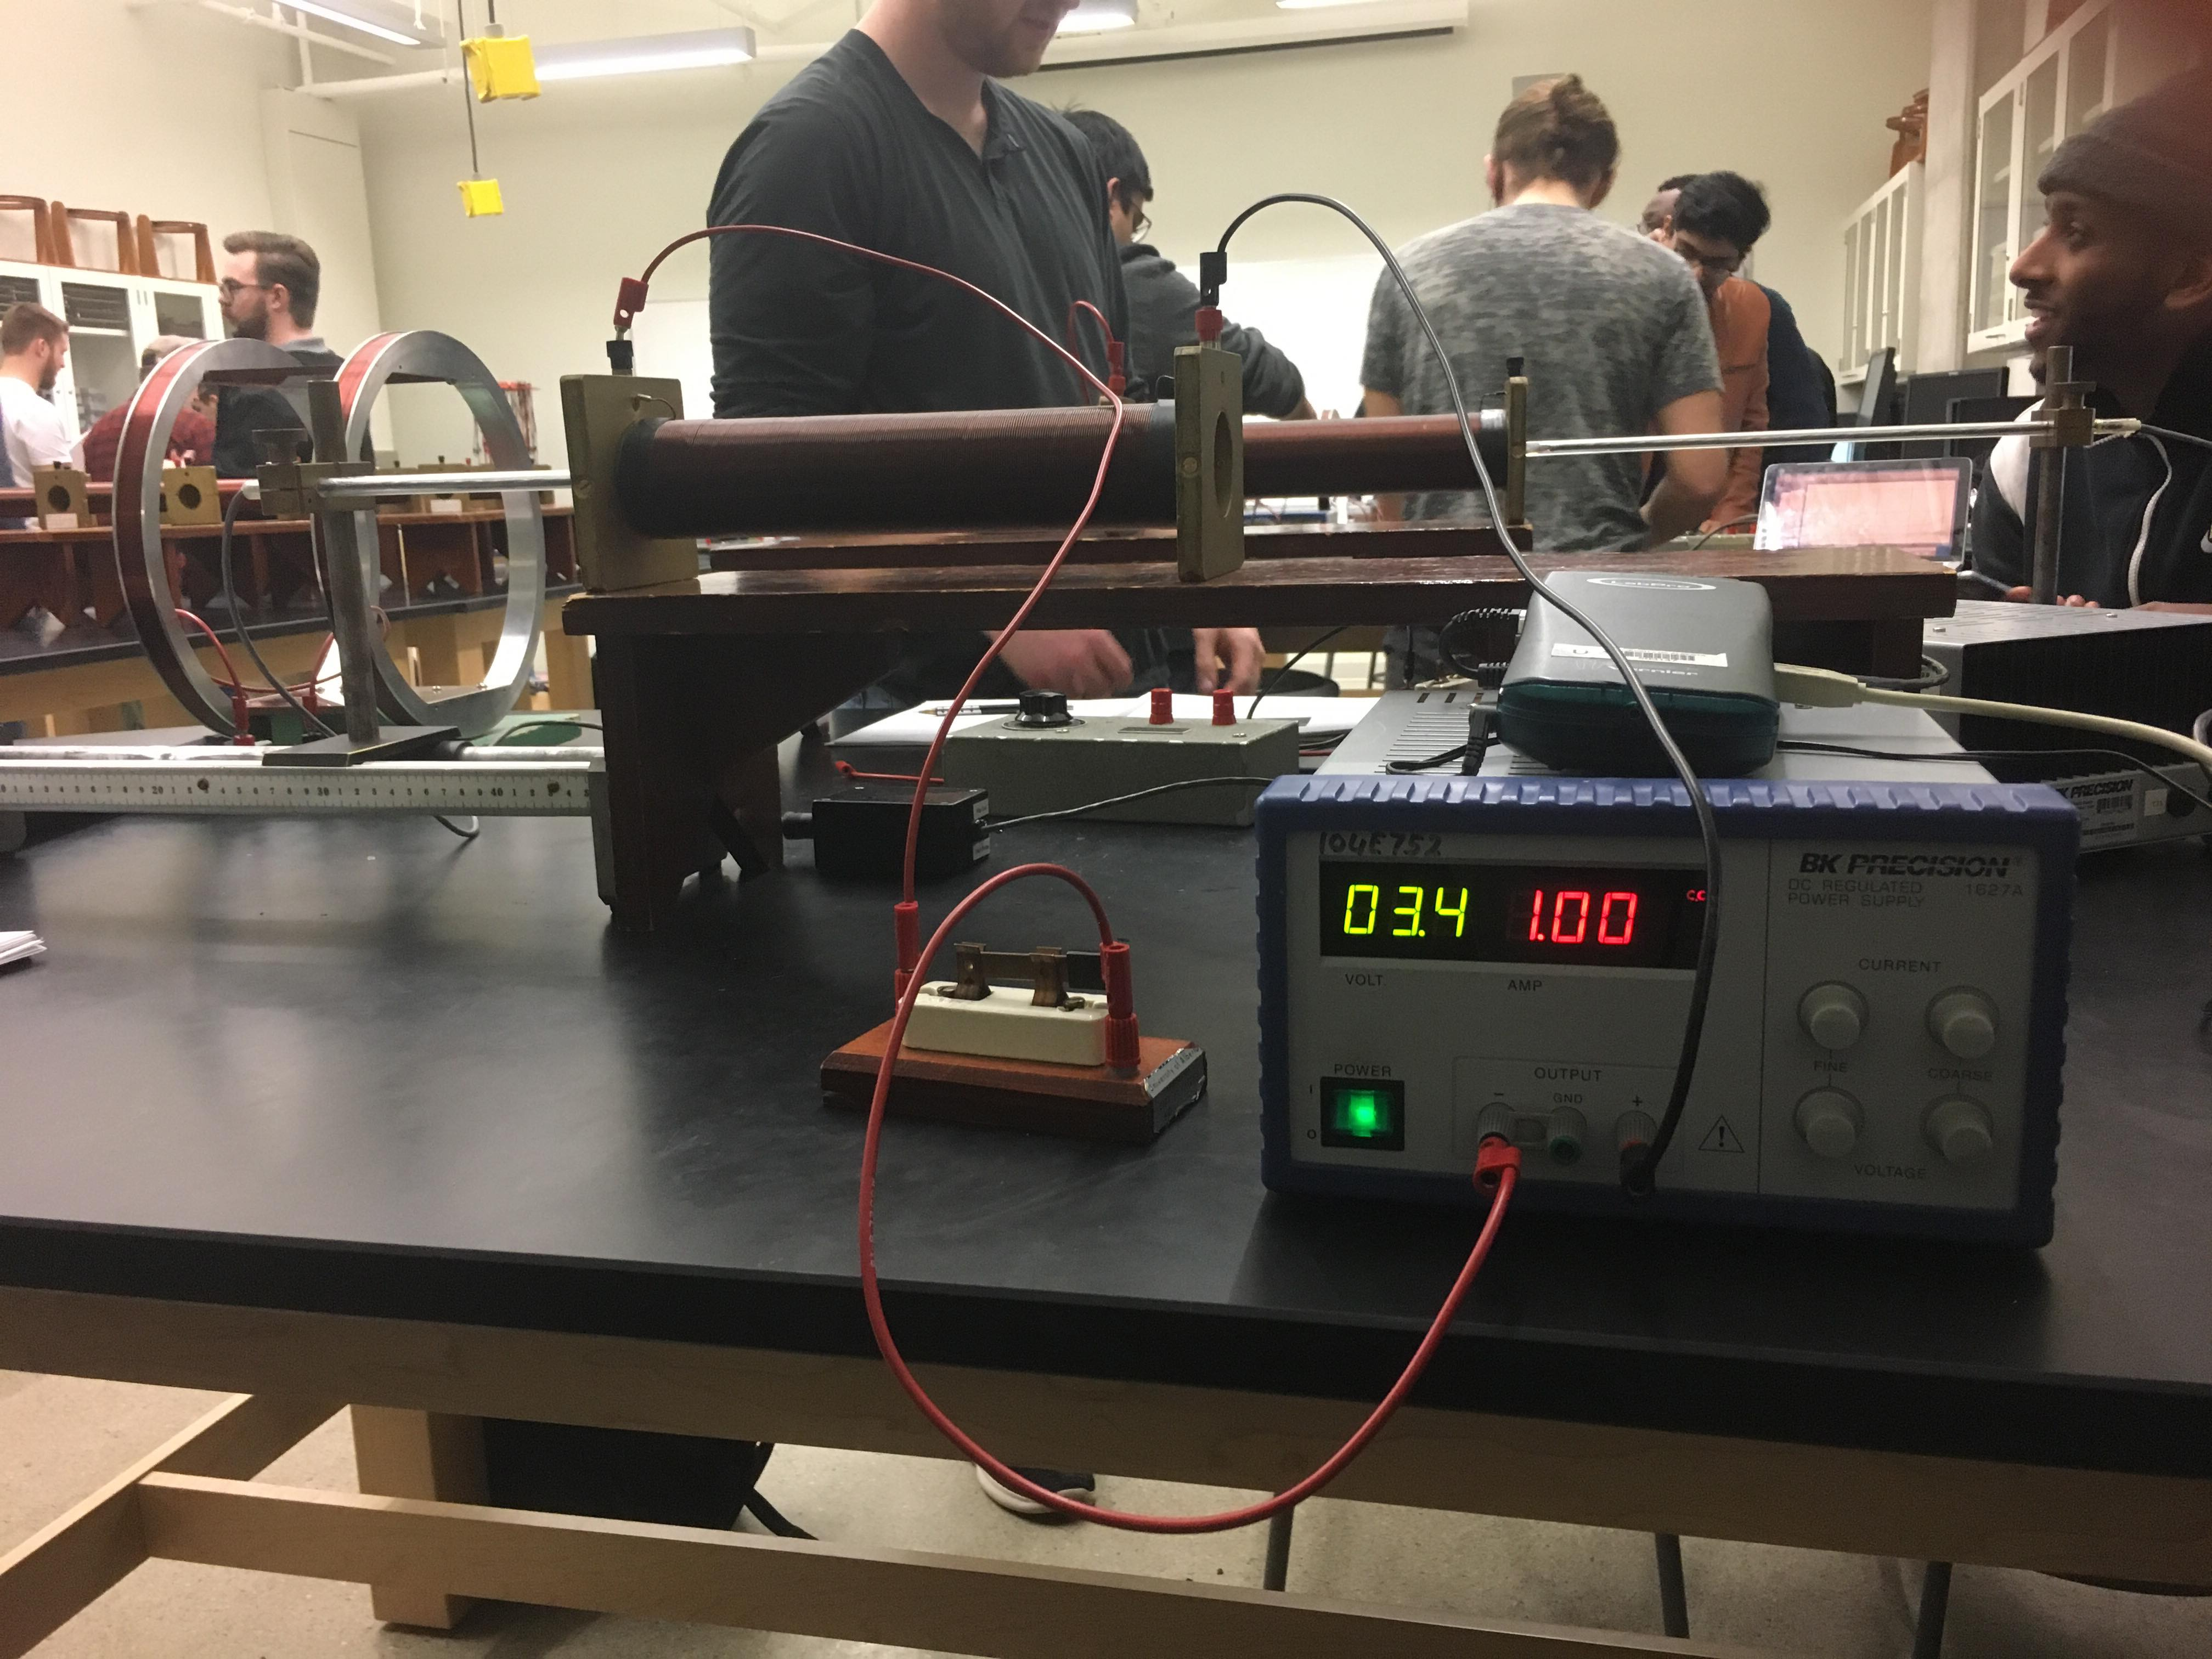
\includegraphics[width=.6\textwidth]{p1-1.jpg}
    \caption{Measuring the magnetic field of a solenoid.}
\end{figure}

The solenoid is wired as shown in Figure 1. Before the circuit is wired up,
$B_E$ is measured using the Hall apparatus. Next, the operating current in the solenoid
was set by setting the current of the power supply to $1.00 A$ with the switch closed.
If a negative value was read for the magnetic field when the switch was
closed and the power supply was on, the current in the solenoid was reversed by switching the
positive and negative leads connected to the power supply. The Hall apparatus
was set up such that the tip of the rod would be just outside of the solenoid,
and centered. From this point, the $B$ field measured in microTeslas was measured
in two centimetre increments as the Hall apparatus was moved inside the coil, until the
tip of the rod just barely reached the end of the coil using LoggerPro software.
Finally, the solenoid length $L$, radius $R$, number of turns $N$, operating current $I$
and ruler position $x_c$ were recorded, and the data was plotted using Excel.

\subsection{Part 2}

\begin{figure}[H]
    \centering
    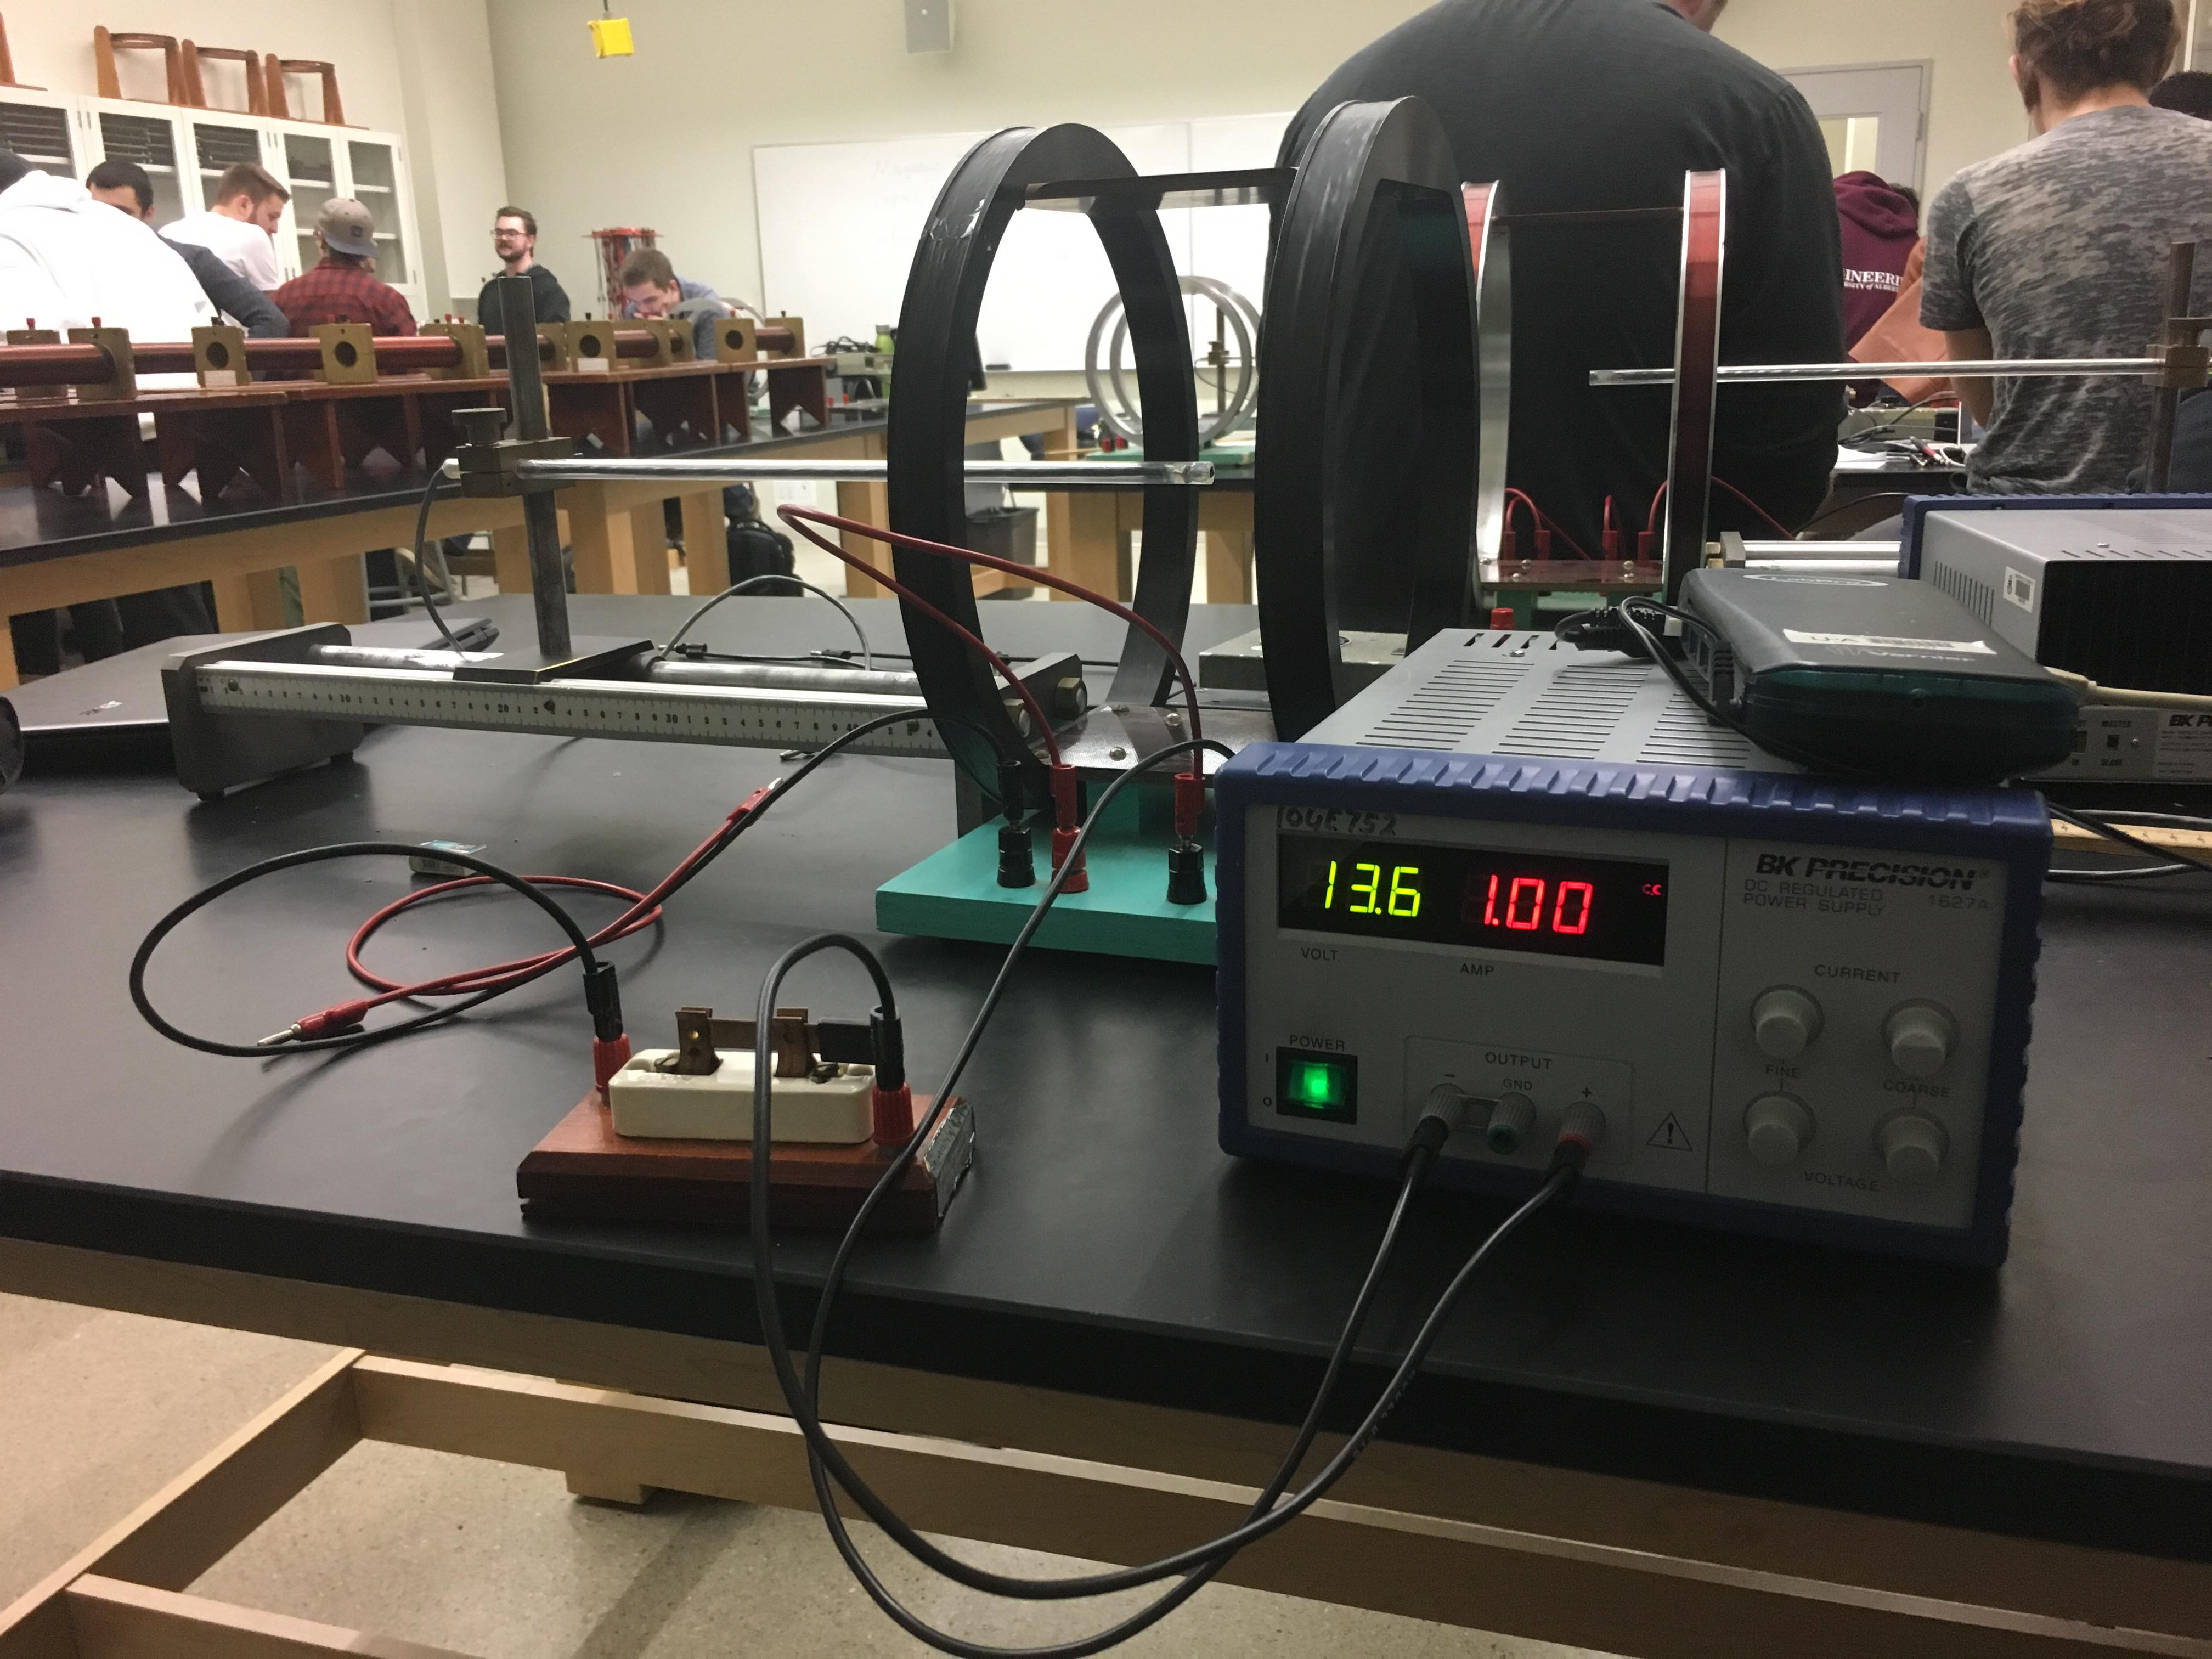
\includegraphics[width=.6\textwidth]{p2-3.jpg}
    \caption{Measuring the magnetic field of the Helmholtz coil.}
\end{figure}
The Helmholtz coils are wired as shown in Figure 2. The tip of the Hall probe
was positioned to be in the exact center of the two coils. Starting at a current
of $0.10 A$, we measured $B_H$ as the current was incremented by $0.1 A$ until
we reached a final current of $1A$. The data was recorded using LoggerPro, and
a graph was generated in Excel.


\section{Results}

\subsection{Part 1}

The constants measured and values calculated used to generate Table 2 are
as follows:

\begin{table}[H]
\centering
\begin{tabular}{ll}
Experimental Constants: & Calculated Constants:     \\ \hline
                        &                           \\
$L =0.280m$             & $\mu_0 =\SI{1.257E-06}{\tesla \metre \per \ampere}$   \\
$R =0.0269m$            & $\mu_0 N I/2/L = \SI{1.70E-03}{\tesla}$ \\
$N = 758$               & $R^2 =0.000724m^2$        \\
$I =1A$                 & $x_c - L/2 =0.111m$       \\
$x_c = 0.251m$          & $x_c + L/2 = 0.391m$      \\
$B_e = -0.257mT$        &                           \\
\end{tabular}
\caption{Experimental and calculated constants}
\end{table}

Table 2 contains the measured values of the magnetic field at verious
positions in the solenoid, as well as calculated theoretical values.

\begin{table}[]
\centering
\begin{tabular}{|c|c|c|c|}
\hline
Measured B (mT) & x (m) & Corrected  $(B - B_E),\pm 2\%$ (T) & Theory $B_t$ \\ \hline
0.50            & 0.099 & 7.57E-04                           & 1.03E-03     \\ \hline
1.40            & 0.119 & 1.65E-03                           & 2.21E-03     \\ \hline
1.99            & 0.139 & 2.25E-03                           & 2.93E-03     \\ \hline
2.19            & 0.159 & 2.45E-03                           & 3.18E-03     \\ \hline
2.26            & 0.179 & 2.52E-03                           & 3.27E-03     \\ \hline
2.27            & 0.199 & 2.53E-03                           & 3.31E-03     \\ \hline
2.25            & 0.219 & 2.51E-03                           & 3.33E-03     \\ \hline
2.25            & 0.239 & 2.50E-03                           & 3.34E-03     \\ \hline
2.25            & 0.259 & 2.51E-03                           & 3.34E-03     \\ \hline
2.26            & 0.279 & 2.52E-03                           & 3.33E-03     \\ \hline
2.25            & 0.299 & 2.51E-03                           & 3.32E-03     \\ \hline
2.23            & 0.319 & 2.48E-03                           & 3.28E-03     \\ \hline
2.18            & 0.339 & 2.44E-03                           & 3.20E-03     \\ \hline
2.02            & 0.359 & 2.28E-03                           & 2.98E-03     \\ \hline
1.56            & 0.379 & 1.82E-03                           & 2.36E-03     \\ \hline
0.65            & 0.399 & 9.11E-04                           & 1.18E-03     \\ \hline
\end{tabular}
\caption{Raw data recorded while measuring $B_s$ as the Hall probe was moved in 2 centimetre increments.}
\end{table}

Using the data in Table 2, a graph is generated, such that we can compare our
experimental data to a theoretical curve.

\begin{figure}[H]
    \centering
    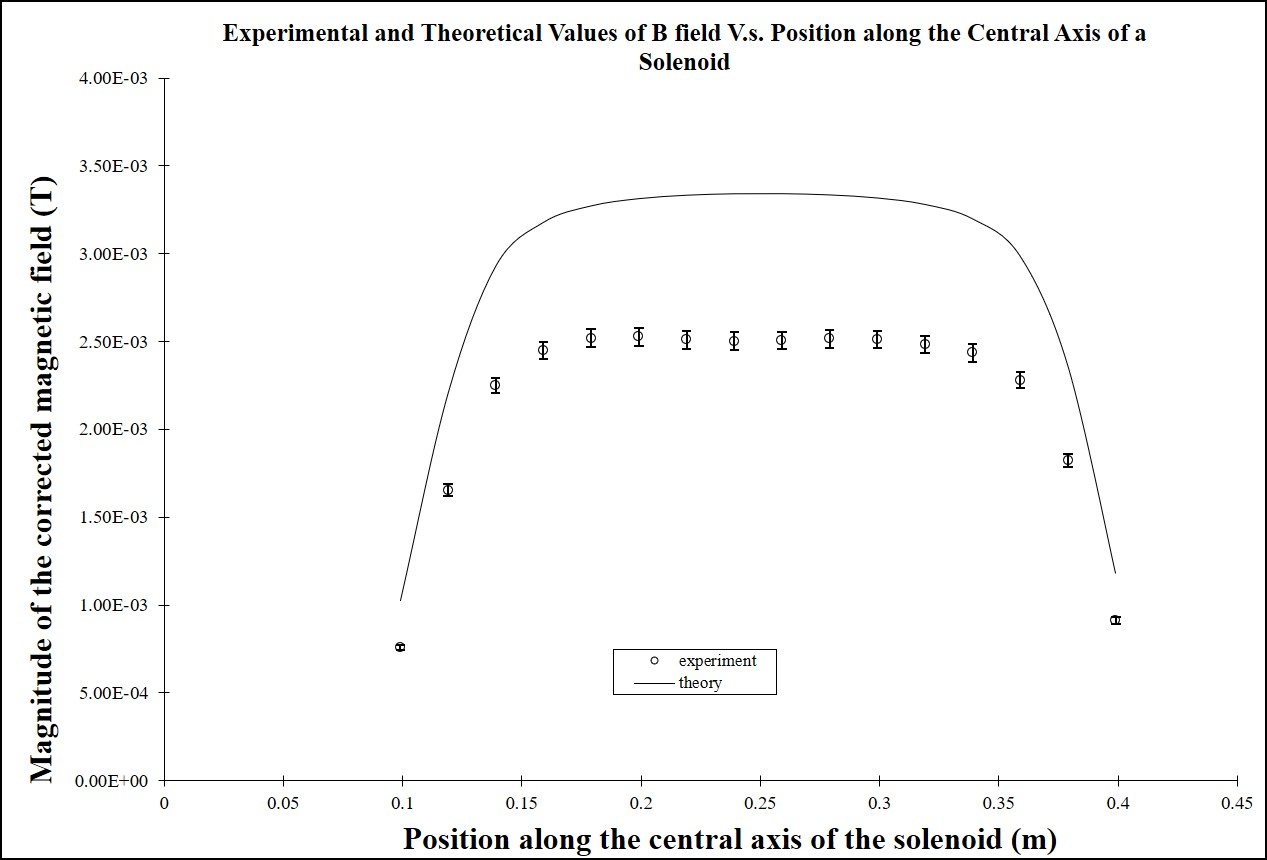
\includegraphics[width=\textwidth]{part1graph.jpg}
    \caption{Experimental values of B field in solenoid compared to theoretical values}
\end{figure}


\subsection{Part 2}



$$ B_H = \frac{8\mu_0NI}{\sqrt{125}R} $$
% $$ \Therefore B_H= \frac{8 (\SI{4\pi e-7}{\tesla\metre\per\ampere})}{\sqrt{125}(\SI{14.8}{\cm})} $$
$$ \Rightarrow N = \frac{B_H \sqrt{125} R}{8\mu_0I} $$
$$ \therefore N= \frac{}{} $$
 so we generate a graph
with $\frac{\sqrt{2V}}{r}$ on the X axis using our measured voltage values, and $B_H$ on the Y axis
using our measured current values.




% \begin{figure}[H]
%   \centering
%   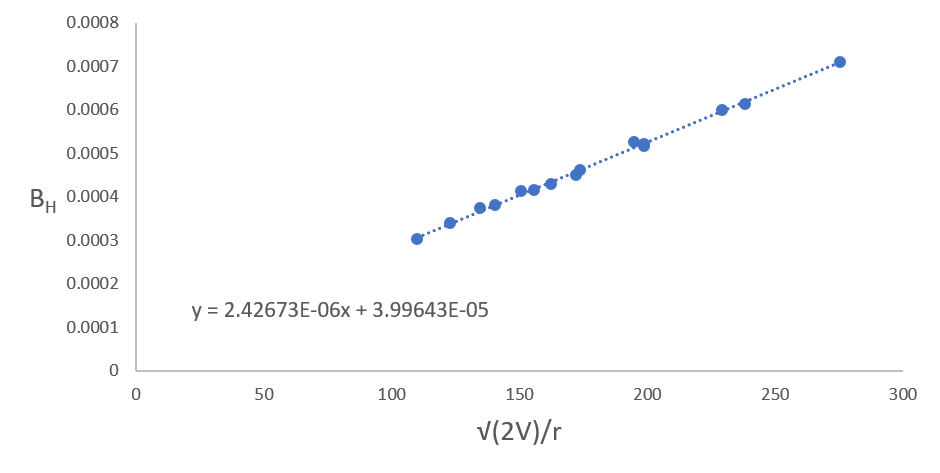
\includegraphics[width=\textwidth]{chart1.png}
%   \caption{Measuring the voltage difference in a region between two parallel conductors.}
% \end{figure}

\newpage
\noindent Using Excel's LINEST function, we obtain the following data from the graph in Figure 3.
\begin{table}[H]
\centering
\begin{tabular}{cc}
  Slope $\sqrt{m/e}$ : &  $\num{2.4267255938411E-06}\pm \num{3.50649774570897E-08}$ \\
  Y-Intercept $B_E$   :&  $\num{3.99642631798173E-05}\pm \num{6.40167504007098E-06}$ \\
\end{tabular}
\caption{LINEST data from the graph in Figure 3}
\end{table}

\noindent To obtain the calculated value for $e/m$, we can see from our LINEST data (Table 2) that the slope, $\sqrt{m/e}$ is
$\num{2.4267255938411E-06}$.\\
Thus, the calculated value of $e/m$ can be found:
$$ \frac{e}{m} = \left(\sqrt{\frac{m}{e}}\right)^{-2} = 1.69808200223924714236 \times 10^{11} $$
And the error $\delta \frac{e}{m}$ can be calculated using partial derivatives:
$$slope= \left(\frac{e}{m}\right)^{-1/2}$$
$$\delta slope = \left| -\frac{1}{2} \left(\frac{e}{m}\right)^{-3/2} \delta \left(\frac{e}{m}\right)\right|$$
$$ 2 \times \delta slope = \left(\frac{e}{m}\right)^{-3/2} \delta \left(\frac{e}{m}\right) $$
$$ \therefore \delta \left(\frac{e}{m}\right) = 2 \times \delta slope \left(\frac{e}{m}\right)^{3/2}$$
From our LINEST data (Table 2), we know that $\delta slope = \num{3.50649774570897E-08} $
$$ \therefore \delta \left(\frac{e}{m}\right) = 2 \times \num{3.50649774570897E-08} \times (\num{1.69808200223924714236e11})^{3/2}$$
$$= \num{4.90728801640585e9} \approx \num{4.91e9}$$
Thus, the calculated value for $\frac{e}{m}$ is:\footnote{Value rounded to three significant digits simply for neatness. Otherwise, the full values were messy and long}
$$\frac{e}{m}=\num{1.70e11} \pm \SI{4.91e9}{\coulomb\per\kilogram}$$
The percent error is:
$$ \frac{|\num{1.69808200223924714236e11}-\num{1.76e11}|}{\num{1.76e11}}\times100 = 3.52\%$$
Obtaining the calculated value and error for $B_E$ is a much simpler matter. We simply
look at the data generated by LINEST, specifically, the Y-intercept (Table 2).
$$B_E = \num{4.00E-05}\pm \SI{6.40E-06}{\tesla}$$
The percent error is:
$$ \frac{|\num{3.99642631798173E-05}-\num{4.8e-5}|}{\num{4.8e-5}}\times100 = 16.74\%$$

\vspace{1cm}
\noindent The calculated values of $e/m$ and $B_E$ from the graph are summarized in Table 3.
\begin{table}[H]
\centering
\begin{tabular}{c|c|c|c|}
                & Expected                      & Calculated:                                     & \% Error \\ \hline
$e/m$: & $\SI{1.76e11}{\coulomb\per\kilogram}$      & $\num{1.70e11} \pm \SI{4.91e9}{\coulomb\per\kilogram}$  &    $3.52$  \\ \hline
$B_E$: & $4.8 \pm \,\SI{0.3e-5}{\tesla}$           & $\num{4.00e-5} \pm \,\SI{6.40e-6}{\tesla}$                    &   $16.74$  \\ \hline
\end{tabular}
\caption{Measured values of $e/m$ and $B_E$ compared to the calculated values obtained from the graph.}
\end{table}

\section{Discussion}

\subsection{Part 1}


From Table 3, we can see that our calculated values for $e/m$
($\num{1.70e11} \pm \SI{4.91e9}{\coulomb\per\kilogram}$)
and $B_E$
($\num{4.00e-5} \pm \,\SI{6.40e-6}{\tesla}$) were in the same order of magnitude as the
expected values. ( $\SI{1.76e11}{\coulomb\per\kilogram}$ for $e/m$
and $4.8 \pm \,\SI{0.3e-5}{\tesla}$ for $B_E$.)
Additionally, the percent error for the charge to mass ration seemed relatively good, being 3.52\%.
However, our calculated value of $B_E$ was a fair bit off, with a 16.74\% error.
Unfortunately, it is clear that our calculated values do are not within error of the
expected values.

At first glance, the graph (Figure 3) produced from our raw data (Table 1) seems reasonable, especially
because all the data points recorded seem to fit nicely on the trendline with
no anomalous data points compared to the other values. This means that whatever error
introduced in our measurement of voltages was a constant factor, since we took care
to measure the currents exactly when the electron loop was on the far side of each peg, as specified in the
lab manual. There are many potential sources of error, including human error, and potential miscalibration of equipment since we are dealing
with electrons which are tiny in nature. We did our best to keep these factors constant.

% \begin{figure}[H]
%   \centering
%   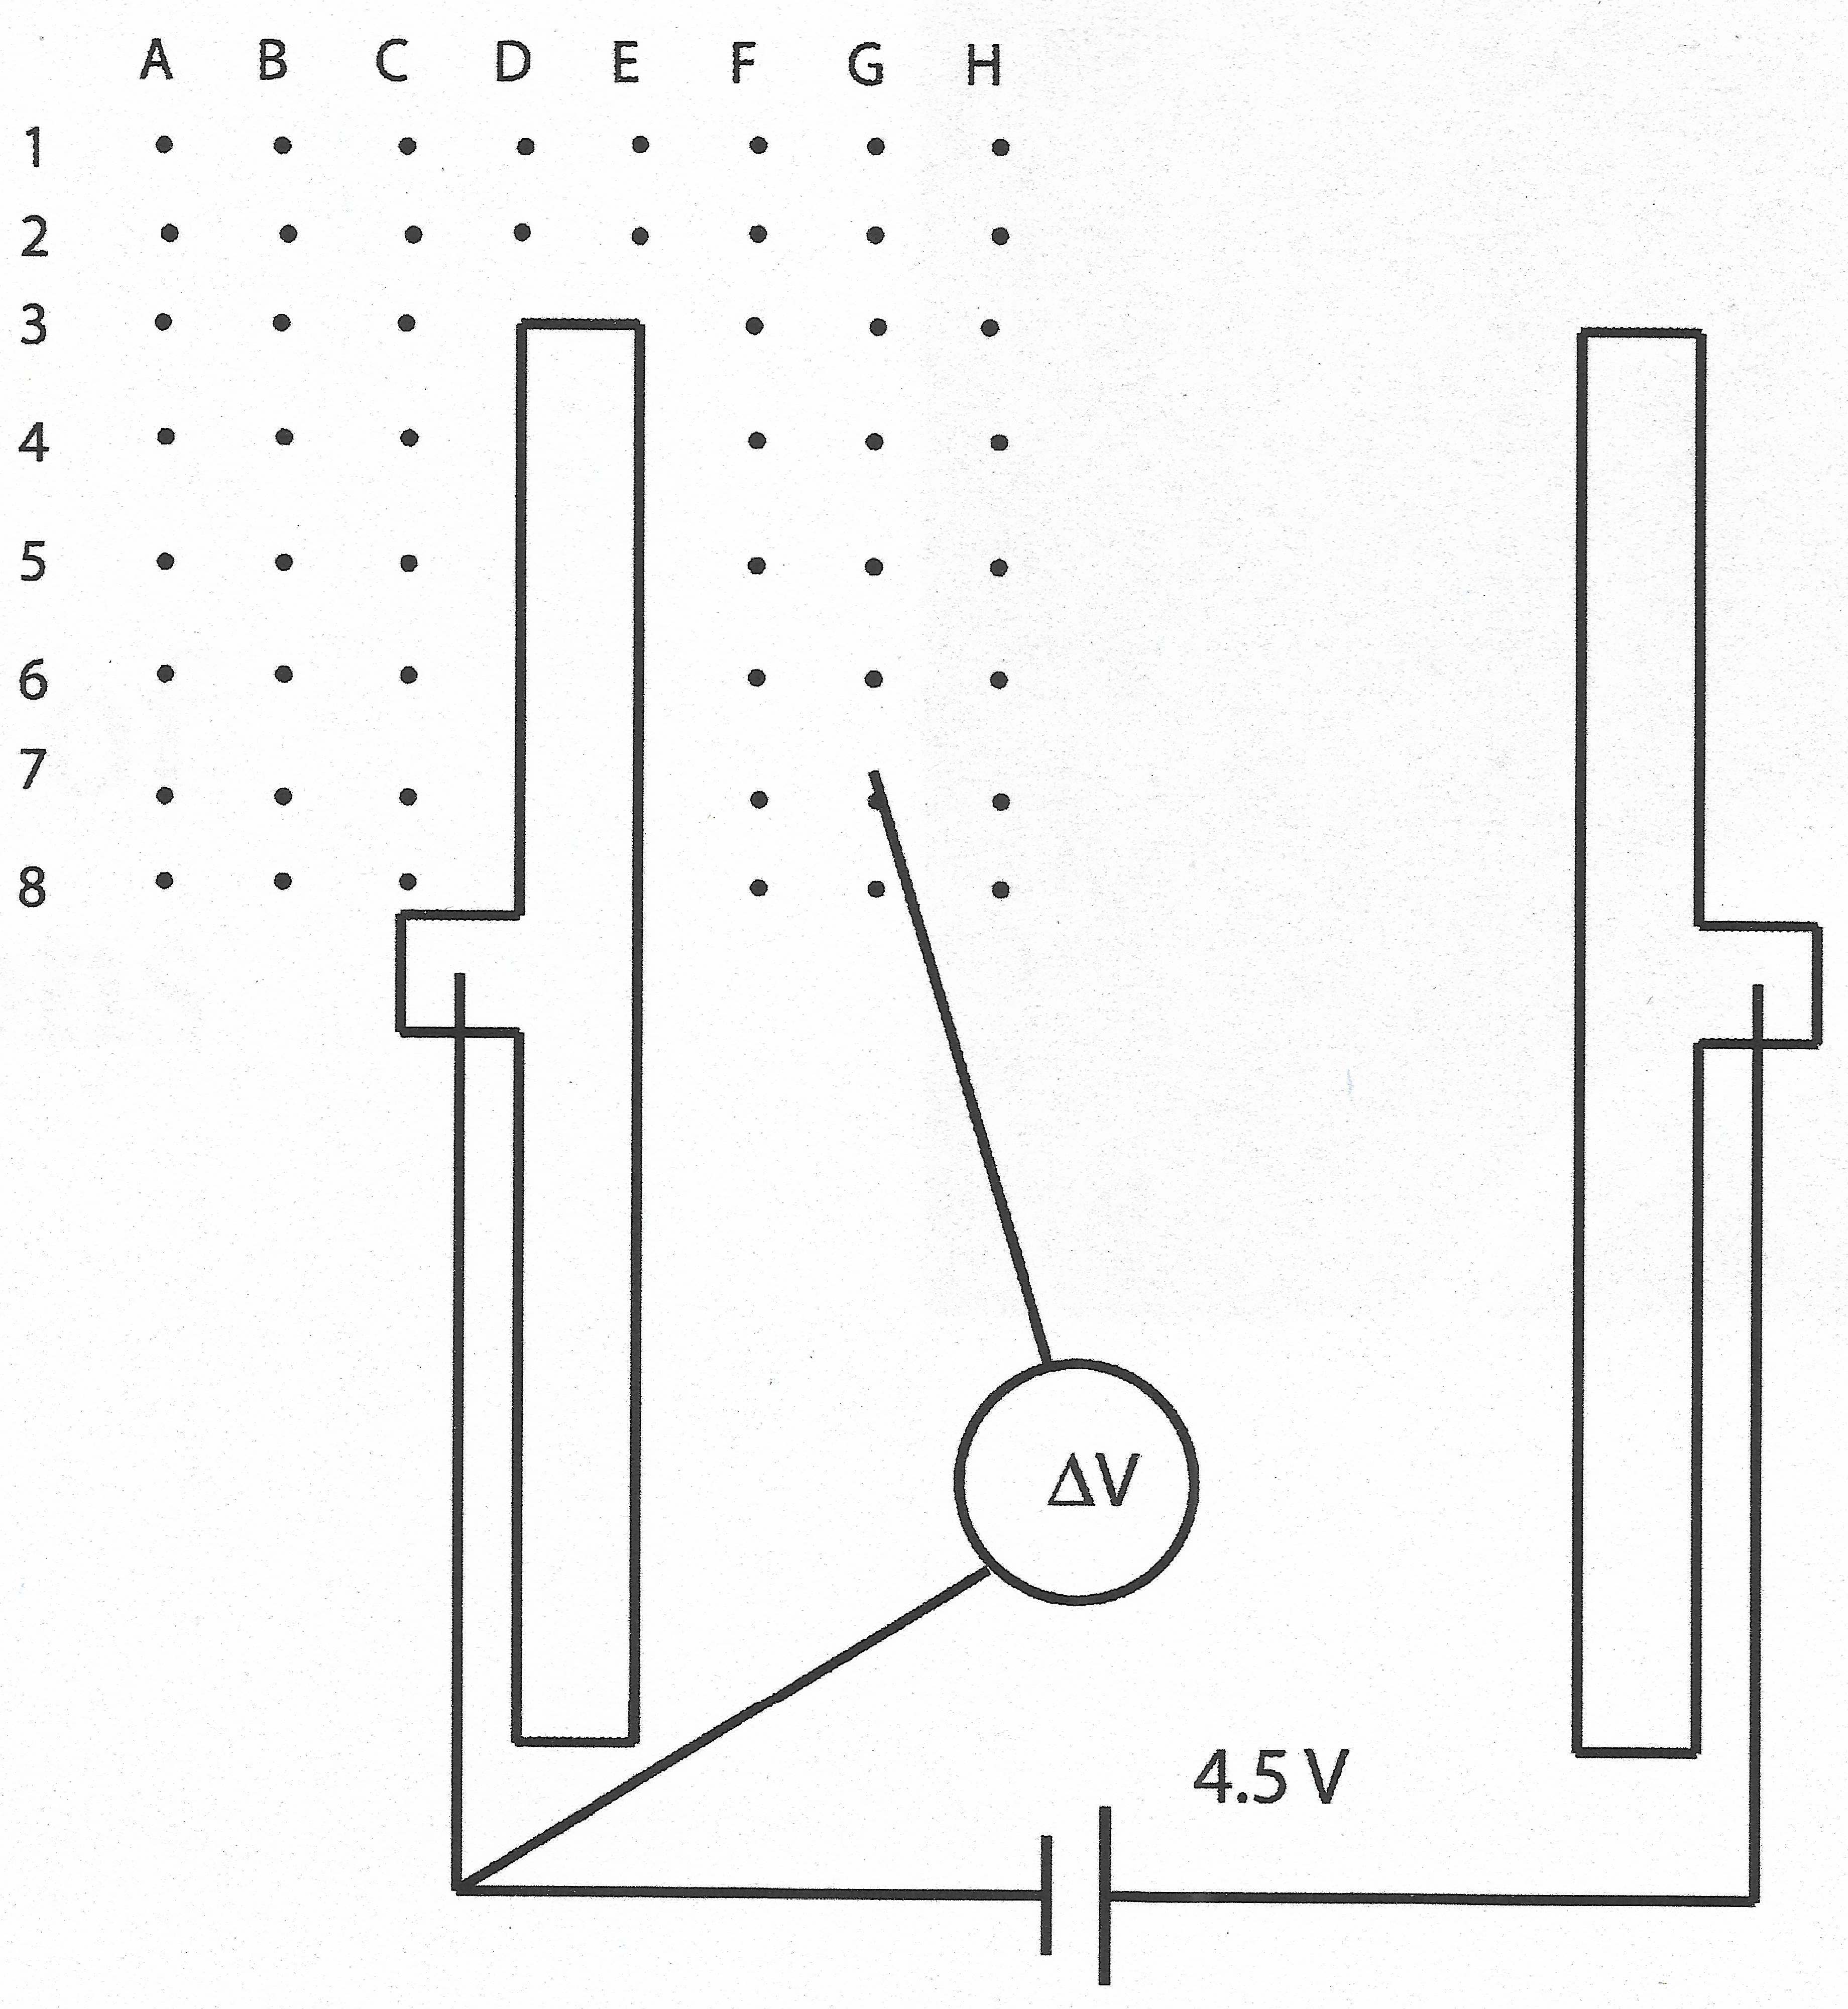
\includegraphics[width=\textwidth]{fig3.jpg}
%   \caption{The direction of the \textbf{B} field is found to be pointing out of the page when drawn this way.}
% \end{figure}

Using the left-hand-rule for moving a charged particle, (since we are
dealing with electrons which have a negative charge), we determine that the net magnetic field \textbf{B}
points upward, perpendicular to the radius of the coil, or upwards relative to Figure 2. Additionally, we notice that
as the Helmholtz current is increased a tighter loop is formed.

Equation 1, which which was manipulated to produce our graph can be derived using the following equations:

\noindent When a stream of electrons are accelerated through a potential difference $V$, the maximum
kinetic energy is given by:
$$\frac{1}{2}mv^2 = eV$$
Next, the Lorentz force \textbf{F} is given by:
$\textbf{F}=q\textbf{v}\times \textbf{B}$
(where $q$ is the charge of the moving particle), and since our magnetic field is set up so that \textbf{B} is perpendicular to the motion of the electrons (see Figure 1),
the magnitude of the force $F$ is given by $$F=qvB$$
Next, the radius of the circle, which is the path of the electrons in this experiment is such that
the centripetal acceleration is furnished by the Lorentz force. Therefore, we obtain $$\frac{mv^2}{r}=evB$$

\noindent To obtain Equation 1, we first rearrange the first of the three equations above and substitute it into the third.
$$\frac{1}{2}mv^2 = eV \Rightarrow v=\frac{\sqrt{2eV}}{m}$$
$$\Rightarrow \frac{m(\frac{2eV}{m})}{r}=e\sqrt{\frac{2eV}{m}}B$$
$$\Rightarrow \frac{4V^2}{r^2}=\frac{2eV}{m}B^2$$
$$\Rightarrow \frac{e}{m} = \frac{2V}{r^2B^2}$$
Finally, we notice that since our apparatus is aimed antiparallel to earth's magnetic field, such that
the magnitude of the total magnetic field $B=B_H-B_E$, and substitute this result in the above equation.
Finally, we obtain equation 1.
$$\frac{e}{m} = \frac{2V}{(B_H-B_E)^2r^2}$$

\textbf{Questions: }\\ \\
\textit{Why is it important to align the Helmholtz coil, so that its field is
        anti-parallel to the earth's magnetic field?}\\
\textbf{A:}
Earth's magnetic field is strong enough to deflect our little electron beam, which means its effects are non-negligible.
However, if we align our Helmholtz coil such that it is exactly anti-parallel to the Earth's magnetic field, we notice that
in this arrangement, since $B_E$ is pointing in the opposite direction to $B_H$, the magnitude of the net magnetic
field can be found simply by subtracting $B_E$ from $B_H$ since
it is anti-parallel to the earth's magnetic field. If the alignment was different, the geometry would not be so simple, and
the path of the electrons would not be in the same plane as the orientation of the Helmholtz coil.\\ \\
\textit{Explain what would happen if the beam in this experiment contained several ions of different masses.}\\
\textbf{A:}
If there were several ions of different masses, the ions with larger mass would
have a larger radius of curvature, and the ions with smaller mass would have a smaller radius of curvature, by observing that
the centripital force depends on the  $F_c=\frac{mv^2}{r}$ relation. By rearranging this, we see that
the mass is directly proportional to the radius of curvature, i.e. $m\propto r$.
Experimentally, we would notice that the glowing path of the ions would be wider, and therefore it would be difficult to measure
the Helmholtz currents exactly at the far side of the pegs in the apparatus, like we did for the electrons, which had unvarying masses.
This ambiguity would also skew our measured charge to mass ratio, since the charged masses are varied and not constant.

\section{Conclusions}
In Experiment 2, we calculate the charge to mass ratio $e/m$ of electrons fired in a Helmholtz coil, which are accelerated by an electric field, and
deflected by a magnetic field to form a circular orbit. The apparatus
was set up such that the magnetic field of the coil is aligned antiparallel to the earth's own magnetic field
to simplify the geomery. The current was varied at three diferent voltages to align the electron loops to known radii, so that we could use the
Helmholtz curents to calculate a value for $e/m$, and the earth's magnetic field $B_E$ by ploting a linear graph. We noticed that the
radius of curvature of the electron loops increased as the Helmholtz current was lowered. Additionally, using the
left hand rule (since electrons are negatively charged masses), we verified that the net magnetic field of the
setup was directed upwards, in the same orientation of the coil (in other words, the direction of the net magnetic field
was perpendicular to the radius of the coil). We calculated the charge to mass ratio of the electron to be ($\num{1.70e11} \pm \SI{4.91e9}{\coulomb\per\kilogram}$)
and the earth's magnetic field to be
($\num{4.00e-5} \pm \,\SI{6.40e-6}{\tesla}$). While these values are in the same order of magnitude as the
expected values ( $\SI{1.76e11}{\coulomb\per\kilogram}$ for $e/m$
and $4.8 \pm \,\SI{0.3e-5}{\tesla}$ for $B_E$), these values do not agree within error. The
graph generated from our data was linear, however, so it is likely that the source of error introduced was a
constant factor, whether it's miscalibration of equipment, or human error since we took care to record our
results in a consistent manner.

\bibliography{references}
\end{document}
